\documentclass[fleqn]{article}

\usepackage{polski}
\usepackage[utf8]{inputenc}
\usepackage[polish]{babel}
\usepackage{parskip}
\usepackage{icomma}
\usepackage[a4paper,includeheadfoot,margin=1.27cm]{geometry}
\usepackage{float}
\usepackage{graphicx}
\usepackage{amsmath}
\usepackage[hypcap=true]{subcaption}
\usepackage{xcolor}
\usepackage{transparent}
\usepackage{listings}
\usepackage[colorlinks=true, linkcolor=blue, pdfborder={0 0 0}]{hyperref}

\renewcommand\thesection{\arabic{section}.}
\renewcommand\thesubsection{\alph{subsection})}
\renewcommand\thesubsubsection{}
\newcommand\square[1]{
	\fcolorbox{black}{#1}{\rule{0pt}{6pt}\rule{6pt}{0pt}}
}

\brokenpenalty=1000
\clubpenalty=1000
\widowpenalty=1000

\title{TM -- Laboratorium 2. \\ \large Licznik 4-bitowy – zerowanie, zliczanie w górę – kod NKB}
\author{Krystian Chachuła \\ Dawid Gruszczyński \\ Marcin Skrzypkowski}

\begin{document}

\maketitle

\setcounter{page}{0}
\thispagestyle{empty}

\pagebreak

\setcounter{page}{1}

\section{Wstęp}

Na drugim laboratorium mieliśmy za zadanie zaprojektować i zrealizować licznik zliczający w górę w kodzie NKB z możliwością asynchronicznego zerowania jego zawartości.
Sterowanie licznikiem miało odbywać się za pomocą dwóch przycisków (CLK aktywne zboczem oraz CLR aktywne poziomem).
Dodatkowym wymogiem zadania była realizacja programowej eliminacji drgań styków oraz zerowania licznika za pomocą przerwania maskowalnego.

Zaprojektowany przed laboratorium układ zbudowaliśmy z następujących układów SML-3:

\begin{itemize}
	\item \textbf{10\_PS1} (moduł zasilacza)
	\item \textbf{100\_LED8} (zestaw 8 diod)
	\item \textbf{120\_IN8} (zestaw 8 monostabilnych wyłączników)
	\item \textbf{202\_NAND} (zestaw bramek \textit{NAND})
	\item \textbf{380\_NOTx6} (moduł sześciu bramek negujących)
	\item procesor Z80 zrealizowany w układzie FPGA
\end{itemize}

\section{Implementacja licznika}

Projektowanie licznika rozpoczęliśmy od stworzenia grafu stanów, który uwzględniał aktywną eliminację drgań styków przycisku zliczającego.
Graf składa się z 4 stanów. W stanie początkowym układ oczekuje na wciśnięcie przycisku, w stanie drugim eliminowane są drgania związanie z wciśnięciem przycisku, w stanie trzecim układ oczekuje na puszczenie przycisku, w stanie 4 eliminowane są drgania związanie z puszczeniem przycisku.
%TODO ogarnąć grafuu

\begin{figure}[H]
	\centering
	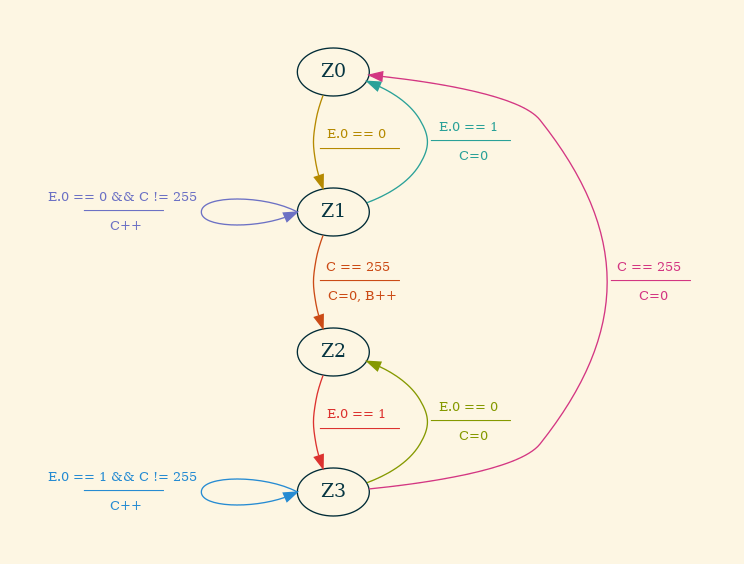
\includegraphics[width=0.72\textwidth]{img/graph.png}
	\caption{Graf automatu stanów}
	\label{fig:graph}
\end{figure}

\textbf{Opis grafu} \\
\\
 W stanie \textbf{Z0} automat czeka na pojawienie się sygnału wciśnięcia przycisku inkrementacji. Sprawdza więc najmniej znaczący bit rejestru E, który służy do przechowywania ostatniej wartości przycisku. Jeśli ma on wartość 0, styki zostały zwarte i automat przechodzi do stanu \textbf{Z1}.\\
 W stanie \textbf{Z1} następuje zliczanie w celu eliminacji drgań przycisku. Każdy obieg pętli głównej programu powoduje inkrementację rejestru C, w którym zliczany jest czas do stabilizacji złącz. Jeśli przed doliczeniem do 255 nastąpi rozłączenie styków, rejestr C jest resetowany, a automat wraca do stanu \textbf{Z0}. Jeśli Przycisk był wciśnięty przez 255 przejść pętli, rejestr C jest resetowany, następuje inkrementacja licznika głównego B odpowiedzialnego za przechowywanie wartości licznika z zadania oraz automat przechodzi do stanu \textbf{Z2}.\\ \\
W stanie \textbf{Z2} automat czeka na puszczenie przycisku. Jeśli najmniej znaczący bit rejestru E jest równy jeden, automat przechodzi do stanu \textbf{Z3}.\\ \\
W stanie \textbf{Z3} Następuje zliczanie obiegów pętli głównej programu z puszczonym przyciskiem. Jeśli styki wciąż są rozwarte, to jest inkrementowany rejestr C. Gdy uzyska on wartość 255, Jest resetowany, a automat przechodzi do stanu \textbf{Z0}. Gdy natomiast przed doliczeniem do tej wartości nastąpi połączenie styków, rejestr C również jest resetowany, ale automat przechodzi do stanu \textbf{Z2}.

Na podstawie stanów automatu powstał kod napisany w języku Assembly.

%TODO  trzeba będzie zrobić opis
\noindent\begin{minipage}{.45\textwidth}
	\lstinputlisting[lastline=50]{src/main.lst}
\end{minipage}\hfill
\noindent\begin{minipage}{.45\textwidth}
	\lstinputlisting[firstline=51]{src/main.lst}
\end{minipage}\hfill
\\
\section{Opis kodu}
Do realizacji zadania licznika wykorzystaliśmy cztery rejestry: B do przechowywania wartości licznika głównego, C do eliminacji drgań przycisku, D do przechowywania stanu automatu, E do przechowywania aktualnego stanu przycisku.
Na samym początku ustawiany jest wskaźnik stosu, tryb obsługi przerwań oraz ustawiane są wartości początkowe odpowiednich rejestrów, następnie następuje  przeskok do pętli głównej programu. \\
Początkowo program znajduje się w stanie \textbf{Z3}, ale gdy przycisk pozostaje niewciśnięty,  automat doliczy w rejestrze C do wartości 255 i wróci do stanu \textbf{Z0}.\\
Z każdym obiegiem pętli głównej jest pobierany najmniej znaczący bit z szyny danych, jego wartośc jest składowana w rejestrze E, do akumulatora ładowany jest aktualny stan automatu. Również na koniec wykonywania instrukcji z każdego stanu następuje przeskok do początku pętli głównej, aby uniknąć blokowania procesora.\\
Na początku każdego stanu program sprawdza, czy znajduje się właśnie w nim. Jeśli tak nie jest, następuje przeskok do następnego. Jeśli w stanie \textbf{Z3} porównanie najmniej znaczących bitów z rejestrem A zwróci wartość 0, program wykona skok do początku pętli głównej.\\
W stanie \textit{s0} następuje załadowanie do akumulatora aktualnego stanu przycisku i sprawdzenie, czy został wciśnięty. Jeśli styki zostały złączone, stan automatu zmienia się na \textbf{Z1}, jeśli nie, następuje powrót do początku pętli głównej.\\
W punkcie \textit{s1} program sprawdza, czy przycisk jest wciąż wciśnięty. jeśli nie jest, następuje reset licznika C, a program wraca do stanu \textbf{Z0}. Jeśli styki wciąż są zwarte, rejestr C jest inkrementowany, następuje sprawdzenie, czy rejestr C doliczył do 255. Jeśli nie, wykonany zostaje skok do początku pętli, jeśli tak, zostaje zinkrementowany licznik główny B i wyświetlana jest nowa jego wartośc, zresetowany rejestr C oraz zmieniony stan automatu na \textbf{Z2}.\\
W punkcie \textit{s2} program sprawdza, czy aktualny stan przycisku uległ zmianie. Jeśli wciąż jest wciśnięty następuje powrót do początku pętli. Jeśli styki zostały rozwarte, następuje przejście do stanu \textbf{Z3}.\\
Punkt \textit{s3} jest analogiczny do \textit{s1}. Następuje porównanie najmłodszych bitów akumulatora oraz rejestru E, jeśli został wciśnięty, następuje powrót do stanu \textbf{Z2}, jeśli w rejestrze C znajdzie się liczba 255, jest on restowany, program ustawia stan \textbf{s0} i wraca do początku pętli głównej.

\textbf{Sekcja krytyczna}
\\
Sekcja krytyczna znajduje się w miejscu inkrementacji licznika głównego. Gdyby w stanie \textit{s1} tuż przed porównaniem wartości rejestru C z wartością 255 nastąpiło przerwanie, które zmienia zawartość akumulatora,po jego zakończeniu mogłaby zostać przyrównana inna wartość, powodując błąd w wyświetlaniu odpowiedniej wartości licznika. Sekcja krytyczna znajduje się również w procedurze \textit{disp}, gdzie w czasie przerwania mógłaby ulec zmianie zawartość rejestru B i zostałaby wyświetlona ponownie zła wartość licznika.
%TODO: opis sekcji krytycznej
\begin{figure}[H]
	\centering
	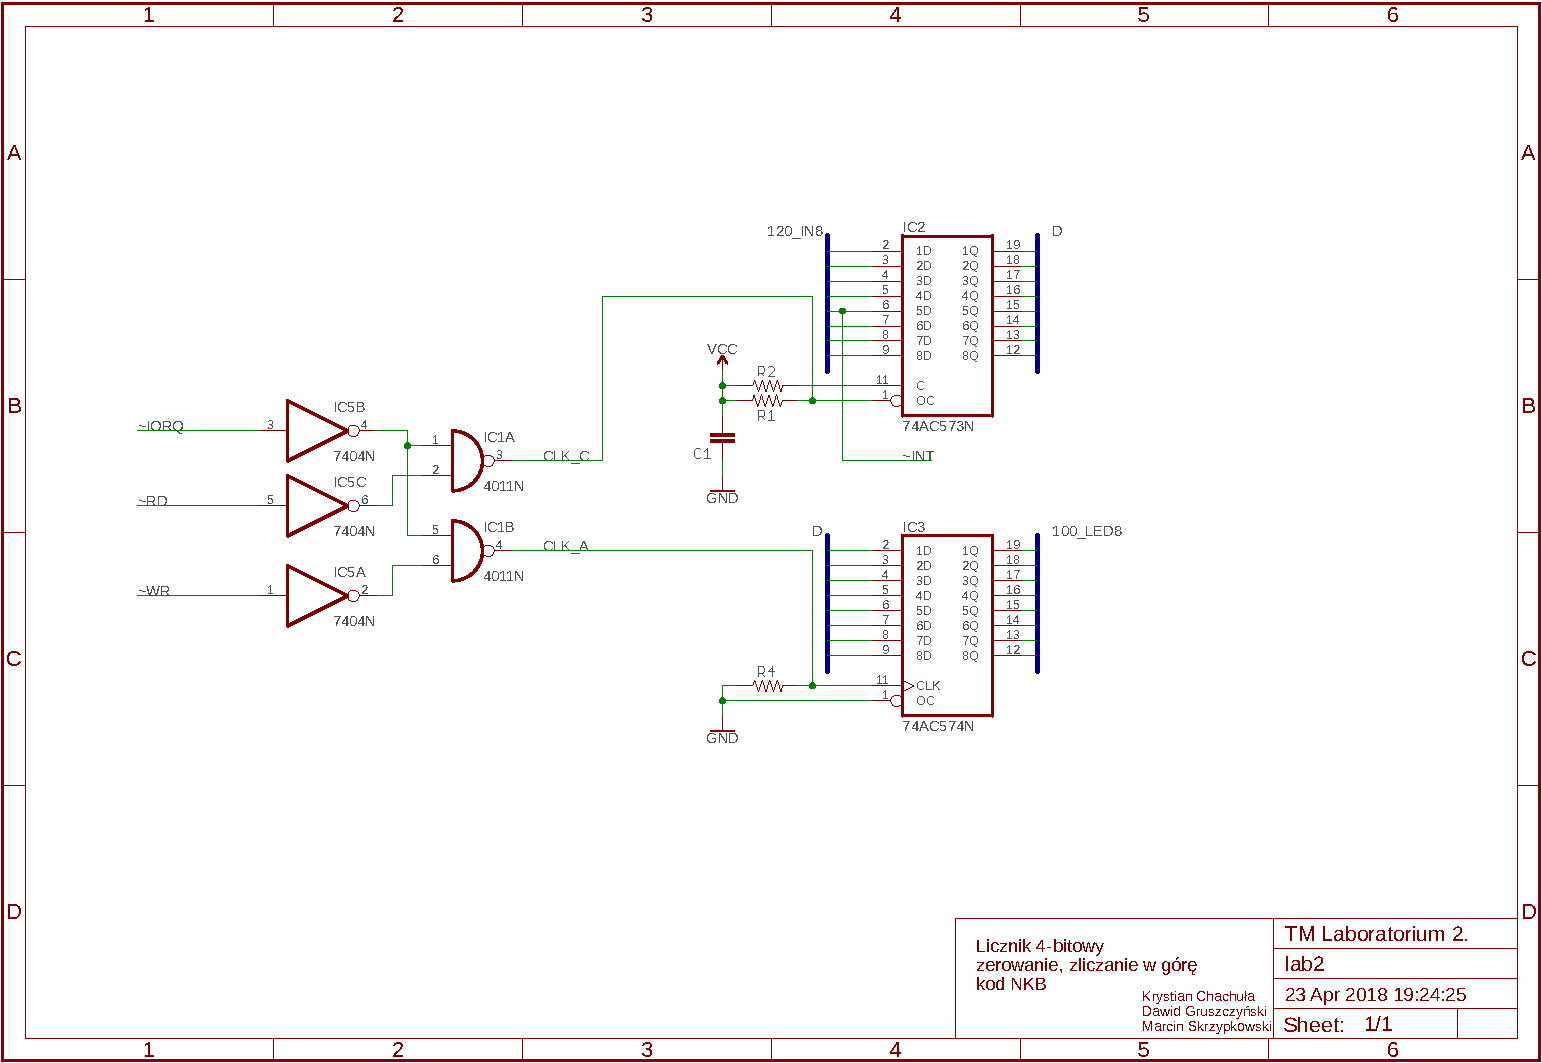
\includegraphics[width=\textwidth]{img/schematic.pdf}
	\caption{Schemat układu}
	\label{fig:schematic}
\end{figure}


Przycisk odpowiedzialny za zliczanie został podłączony do wejścia D0 rejestru wejściowego C, natomiast przycisk odpowiedzialny za asynchroniczne zerowanie do wejścia $\overline{INT}$ procesora.
Wyświetlanie zawartości licznika odbywa się za pomocą rejestru wyjściowego A, którego wyjścia podłączone są do modułu diod SML-3 $\textit{100\_LED8}$. Rejestry A i C podłączone są do procesora w taki sposób by reagowały tylko na operacje zapisu do przestrzeni wejścia/wyjścia (rejestr B) lub odczytu (rejestr C), a więc wyświetlanie zawartości oraz odczyt stanu przycisku zliczającego.


\section{Problemy}
W trakcie pracy nad licznikiem natrafiliśmy na problem związany z organizacją programu w przestrzeni pamięciowej procesora Z80. Aby zdefiniować procedurę obsługi przerwania (tryb 1.) użyliśmy w kodzie polecenia \lstinline|ORG 1838h|, lecz po złożeniu i konwersji przez narzędzie \textit{bin2hex} program nie zachowywał się zgodnie z naszymi oczekiwaniami. Poleceniem którego szukaliśmy było \lstinline|DS 0x1838-$, 0|, które wypełnia bajty do adresu 1838 zerami (instrukcjami \lstinline|NOP|). Dzięki temu następne linie kodu były wykonywane jako \textit{ISR}.
\end{document}
